\documentclass[11pt,a4paper]{report}

\usepackage{amssymb,amsmath,epsfig,float,subfig,hyperref,multicol}

\usepackage{xcolor}

\definecolor{SCSUred}{HTML}{CD1041}

\hypersetup{colorlinks=true,linkcolor=SCSUred,urlcolor=SCSUred}

\usepackage{enumerate}
\usepackage{tikz}
\usetikzlibrary{arrows}
\usetikzlibrary{patterns}
\usetikzlibrary{decorations}
%%\usetikzlibrary{intersections}
\usetikzlibrary{matrix}
\usetikzlibrary{snakes}
\usetikzlibrary{calc}
\usetikzlibrary{backgrounds}

\definecolor{linecolor}{HTML}{0074C8}
\definecolor{linecolor2}{HTML}{C80200}

\newcommand{\imagebullet}[1]{\includegraphics[width=0.5cm]{#1}}

\pagestyle{empty}
\setlength{\textwidth}{7in}
\setlength{\textheight}{10in}
\setlength{\oddsidemargin}{-25pt}
\setlength{\evensidemargin}{-25pt}
\setlength{\topmargin}{-50pt}

\usepackage[english]{babel}
\usepackage[utf8]{inputenc}
\usepackage{fancyhdr}
 
%%\pagestyle{fancy}
\renewcommand{\headrulewidth}{0pt}
%%\fancyhf{}
%%\rhead{Share\LaTeX}
%%\lhead{Guides and tutorials}
%%\cfoot{OVER}

\newcommand{\DueA}{Tuesday, October 29}
\newcommand{\DueB}{Thursday, October 31}
\newcommand{\DueC}{Thursday, November 7}

\begin{document}

\begin{figure}[ht]
\begin{flushright}
	\includegraphics[width=2.0in]{U_PriHorz_WhtLtBG.jpg}
	\end{flushright}
\end{figure}

\vspace{-12mm}

\begin{flushleft}
\Large\bf \href{https://activecalculus.org/single/sec-3-4-applied-opt.html}{3.4 - Applied Optimization}\rm
%%Daily Preparation - \DueA \rm
\end{flushleft}


\vspace{8pt}

\noindent {\Large\bf{Overview}} \\
The derivative of a function tells us key information.  We now investigate the concept of optimization. That is, we are interested in determining where the value of a function is greatest or least, and the input value(s) at which such extremes occur. As we move from Section 3.3 into Section 3.4, we start to emphasize problems that occur in a more applied setting, ones that are based in some sort of physical reality. Here, you will be challenged to read carefully and interpret different possible scenarios, identify variables and determine functions, and to use calculus to justify the reasoning behind your ultimate answers.




\vspace{16pt}

%%\pagebreak

\noindent {\Large\bf{To prepare for class}} \\
Complete all actions listed below.  Respond to the questions highlighted with {\color{SCSUred}{\boxed{Submit}}}.  %% by the start of class on {\bf{\DueA}}.  A single .pdf should be uploaded to D2L Brightspace. 
\begin{itemize} \itemsep -2pt % Reduce space between items

\item {\bf{Read}} motivating questions and the introduction to \href{https://activecalculus.org/single/sec-3-4-applied-opt.html}{section 3.4} (up until Preview Activity 3.4.1).

\item[{\color{SCSUred} \boxed{Submit}}]  {\bf{Do}} \href{https://activecalculus.org/single/sec-3-4-applied-opt.html#uUz}{Preview Activity 3.4.1}.  
\begin{itemize} \itemsep -2pt % Reduce space between items
\item After completion, look back by using \href{https://www.geogebra.org/classic?lang=en}{GeoGebra} to graph the function $f(x) = x^2(108-4x)$ on $[0,27]$.  How does this graph relate to your solution to the problem? 
\item (Optional) {\bf{Watch}} \href{https://www.youtube.com/watch?v=vFjZWP1Jotc}{video solution to Preview Activity 3.4.1}.  
\end{itemize}

\item {\bf{Read}} \href{https://activecalculus.org/single/sec-3-4-applied-opt.html#FNq}{section 3.4.1} on steps used to solve an applied optimization problem.

\item {\bf{Watch}} video \href{https://www.youtube.com/watch?v=Ilu2SZa3SYA&feature=emb_title}{Quick Review - Applied Optimization (2:14)}.

\item {\bf{Watch}} video \href{https://www.youtube.com/watch?v=jH6J-n6zt4c&list=PL9bIjQJDwfGuXQHuS5Jkmum_CFILoCZX-&index=70}{Fencing Optimization (7:08)}.

  


\item {\bf{Do}} these problems.
\begin{enumerate}
\setcounter{enumi}{1}

\item[{\color{SCSUred} \boxed{Submit}}] 1. If you have 100 feet of fencing and want to enclose a rectangular area up against a long, straight wall, what is the largest area you can enclose?  

\item[\imagebullet{CopilotLogo.jpg}] Prompt {\bf{Copilot}} ``If you have 100 feet of fencing and want to enclose a rectangular area up against a long, straight wall, what is the largest area you can enclose?   Explain."  Does the AI get this question correct?  Does it even use calculus to `solve' the problem?  

\item Find a positive number such that the sum of the number and twice its reciprocal is as small as possible.

\item[\imagebullet{CopilotLogo.jpg}] Prompt {\bf{Copilot}} ``Find a positive number such that the sum of the number and twice its reciprocal is as small as possible.  Explain."  Follow up the response by prompting ``But just because the derivative is 0 does not make this value a minimum.  So why do you claim it is?"  Does the AI give useful and correct feedback?  

\item A vertical line divides a triangle into two pieces.  \\
Find the value of the coordinate $x$ that maximizes the product of the two areas.  \\
{\it{Hint: The function $A(x)$ you seek to maximize on domain $[0,1]$ \\ is the product of the area of the ``smaller'' triangle and what remains.  \\ The area of what remains is simply the area of the large triangle \\ minus the area of the small triangle.}}
\vspace{-30mm}
 \begin{figure}[H]
\flushright
{
  \begin{tikzpicture}[thick,scale=2.5] [domain=-1:2]
   \draw [black, dotted, line width=1pt] (0.7,0) -- (0.7, 1.4) node [below] at (0.7,-0.1) {$x$};
   \draw [black] node [below] at (1,-0.1) {$1$};
      \draw [black] node [below] at (0,-0.1) {$0$};
      \draw [black] node [right] at (1,1) {$2$};
%%\draw[color=linecolor, line width=1.5pt,domain=0.5:6.5]   plot (\x,{0.25*(\x-1)^2-1});
\draw [linecolor, line width = 1.5pt] (0,0) -- (1,0) -- (1, 2) -- (0,0);

\end{tikzpicture}}  
\end{figure}


 
\end{enumerate}
  
\item[{\color{SCSUred} \boxed{Submit}}] {\bf{Do}} \href{https://activecalculus.org/single/sec-3-4-applied-opt.html#zsk}{exercise 1 in section 3.4}.  Submit a screen capture of a ``check of the answers'' to your work.  Also, answer these two questions:
\begin{itemize}
\item What is the function $V(x)$ that you are seeking to maximize?
\item On what domain are you looking for the maximum of $V(x)$?  
\item What does {\it{GeoGebra}} produce when you graph $V(x)$ on this domain?
\end{itemize}
If you would like to visualize a similar problem, \href{https://www.geogebra.org/m/jqbgveyd}{this applet} may help.  \\
If you would like a hint, Khan Academy as a video you can watch that explains how to do a similar problem (though without {\it{GeoGebra}} and with different dimensions given.  See \href{https://www.khanacademy.org/math/ap-calculus-ab/ab-diff-analytical-applications-new/ab-5-11/v/optimizing-box-volume-graphically}{Optimization: Box Volume (Part I)} and \href{https://www.khanacademy.org/math/ap-calculus-ab/ab-diff-analytical-applications-new/ab-5-11/v/optimizing-box-volume-analytically}{Optimization: Box Volume (Part II)}.  He makes mistakes (such as not using an approximation symbol when he should), but the solution process is reasonable.  

\item {\bf{Do}} \href{https://activecalculus.org/single/sec-3-4-applied-opt.html#zsk}{exercises 2-5 in section 3.4}. 

\end{itemize}























\vspace{16pt}

\noindent {\Large\bf{After class}}\\
Solidifying the concepts discussed in class through practice is necessary to build your skills. 

%%\noindent {\large\bf{After \DueA}}
\begin{itemize}\itemsep -2pt % Reduce space between items

\item {\bf{Watch}} video \href{https://www.youtube.com/watch?v=uJFxdxSBjok&feature=emb_title}{Optimization with Trigonometry (13:24)}. 

%%\item {\bf{Do}} \href{https://activecalculus.org/single/sec-3-4-applied-opt.html#LZK}{Activity 3.4.2}.  After completion, look back by using \href{https://www.geogebra.org/classic?lang=en}{GeoGebra} to graph the function $$\displaystyle f(x) = (0.027)2\pi x^2 + (0.015)2\pi x\frac{16}{2\pi x^2}$$ on $(0,15).$  How does this graph relate to your solution to the problem?

\item {\bf{Read}} \href{https://activecalculus.org/single/sec-3-4-applied-opt.html#lUz}{section 3.4.2 - summary}.

\item {\bf{Do}} \href{https://activecalculus.org/single/sec-3-4-applied-opt.html#Ecd}{exercises 6-7 in section 3.4}.


%%\item {\bf{Do}} the following problem.
%%\begin{enumerate}
%%\setcounter{enumi}{3}


%%\item A rectangular beam is cut from a cylindrical log \\ of radius 30 cm.  The strength of a beam of width $w$ \\ and height $h$ is proportional to $wh^2$.  \\ Find the width and height of the beam of \\ maximum strength.  

%%\vspace{-40mm}
%% \begin{figure}[H]
%%\flushright
%%{
%%  \begin{tikzpicture}[thick,scale=1] [domain=-1:2]
%%\draw [linecolor, line width = 1.5pt] circle (3);
%%\draw [black, line width= 1pt] (0,0) -- (2.5,1.66) node [above] at (1,0.8) {$30$};
%%\draw [linecolor, line width = 1.5pt] (2.5,1.66) -- (2.5,-1.66) -- (-2.5, -1.66) -- (-2.5,1.66) -- (2.5, 1.66);
%%\draw [black] node at (-2.25, 0) {$h$};
%%\draw [black] node at (0,-1.4) {$w$};
%%\fill [black] (0,0) circle (3pt);
%%\end{tikzpicture}}  
%%\end{figure}



%%\end{enumerate}

%%\end{itemize}

%%\noindent {\large\bf{After \DueB}}

%%\begin{itemize}

%%\item {\bf{Do}} \href{https://activecalculus.org/single/sec-3-4-applied-opt.html#YXW}{Activity 3.3.4}. 

\item {\bf{Do}} \href{https://activecalculus.org/single/sec-3-4-applied-opt.html#Qqv}{exercises 8-9 in section 3.4}.

\item {\bf{Watch}} video \href{https://www.youtube.com/watch?v=_Y7XJEdEkAE}{Minimum-time hiking route, part 1 (8:35)}.  Then, {\bf{watch}} video \href{https://www.youtube.com/watch?v=2Fuf1epEjhk}{Minimum-time hiking route, part 2 (8:40)}.  



\item {\bf{Do}} this problem.
\begin{enumerate}
\setcounter{enumi}{3}

\item Alaina wants to get to the bus stop as quickly as possible.  The bus stop is across a grassy park, 2000 feet west and 600 feet north of her current position.  Alaina can walk west along the edge of the park on the sidewalk at a speed of 6 ft/sec.  She can also travel through the grass in the park, but only at a rate of 4 ft/sec.  

\begin{figure}[H]
\begin{center}
	\includegraphics[width=5.0in]{fig_04_31.jpg}
	\end{center}
\end{figure}

\vspace{-10mm}
\begin{enumerate}
\item Of the paths shown in the diagram above, the one in (a) is the shortest in length and the one in (b) is the longest in length.  Which one of these three is the {\it{shortest in time}}?  
%%\vspace{40mm}
\item If Alaina walks $x$ feet west along the sidewalk before heading diagonally across the park to the bus stop, the total time it takes her will be $T = T_{sidewalk} + T_{park}$.  Write $T$ as a function of $x$.  
%%\vspace{70mm}
\item What is the domain of the function $T$ found in part (b)?  For what value of $x$ on this domain is this function minimized?  What is the minimum value?  {\it{GeoGebra may be used to help estimate this value.}}
\end{enumerate}

%%\item An aluminum can (in the shape of a cylinder) is to be designed to hold 64 cm$^3$ of juice.  The aluminum on the top and the bottom is twice as thick (and hence twice as costly) as that on the side of the can.  What are the dimensions that minimize the cost of construction? 


\end{enumerate}


\item {\bf{Start working}} on the \href{https://www.myopenmath.com/index.php}{MOMwork} (MyOpenMath) assignment for this section.  %%This will be due on \DueC. 

\end{itemize}

\pagebreak

\vspace{16pt}

\noindent {\Huge\bf{Extra Prep}}


\vspace{16pt}

\noindent {\Large\bf{Basic learning objectives}}\\
These are the tasks you should be able to perform with reasonable
fluency when you arrive at our next class meeting. Important new
vocabulary words are indicated {\it{in italics}}.  Check each box when you feel confident you have a firm grasp on that objective.

\begin{itemize} \itemsep -2pt % Reduce space between items
\renewcommand{\labelitemi}{\scriptsize$\square$}
\item (Review) Determine where to look for extreme values of a function on a closed interval, and what we need to do when the interval is open.
\item Identify and classify all critical values of a function (within any given domain of interest).

\item Through problems such as Example 3.4, recognize how we often need to introduce a function in order to optimize some quantity of interest:
\begin{itemize}
\item Identify the variables in the problem as well as the constraints on the variables.

\item Identify the ``target quantity", i.e. the quantity to be optimized.

\item Set up an equation to relate the target quantity to the other variables.

\item Use a constraint in the problem to reduce the number of other variables in the equation to one, and solve for the target quantity to obtain a function of one variable.
\end{itemize}
\end{itemize}

\vspace{16pt}

\noindent {\Large\bf{Advanced learning objectives}}\\
In addition to mastering the basic objectives, here are the tasks you should be able to perform after class, with practice:
\begin{itemize} \itemsep -2pt % Reduce space between items
\renewcommand{\labelitemi}{\scriptsize$\square$}
\item In a wide range of contexts, identify and formulate a function of interest and then use calculus to accurately justify where the function is optimized on an appropriate domain.
\end{itemize}

\vspace{16pt}

\noindent {\Large\bf{Need More Help?}}

\begin{itemize}\itemsep -2pt % Reduce space between items
\item  {\bf{Watch}} another video on another version of the very famous ``Farmer and the Fence'' problem: \href{https://www.youtube.com/watch?v=QCFObvt7YOg&feature=youtu.be}{How to Maximize the Area of a Rectangular Pen (5:56)}.
\end{itemize}

\vspace{16pt}

\noindent {\Large\bf{Selected Answers}}
\begin{enumerate}
\setcounter{enumi}{0}

\item 1250 square feet\\
Our goal is to maximize $A(x,y) = xy$ where $x$ represents the length of two sides of fence and $y$ is the length of the other (the length parallel to the wall being used).  We maximize $A(x,y)$ subject to the condition that $2x+y=100$.  By solving for $y$, we aim to maximize $$A(x)=x(100-2x) = 100x-2x^2$$ on the domain $0 \leq x \leq 50$ (because $0 \leq y=100-2x \leq 100$).  Since $A'(x) = 100-4x$ we find a critical value at $x=25$ that leads to a global maximum of $A$ on its domain.  $A(25) = 1250$.  

\item The positive number is $\sqrt{2}$. The function $Q(x)$ being minimized is $Q(x) = x + \frac{2}{x}$.  It is being minimized on the domain $(0,\infty)$.  Since $Q'(x) = 1-2x^{-2} = 1-\frac{2}{x^2} = 0$ exactly when $x=\pm \sqrt{2}$, we see that $\sqrt{2}$ is the only critical point in the domain.  A first derivative sign chart shows us that this is a local minimum.  

\item We maximize $$A(x) = \frac{1}{2}x(2x) \cdot \left[ \frac{1}{2}(1)(2) - \frac{1}{2}x(2x)\right] = x^2 [1-x^2]$$ on the interval $0 \leq x \leq 1$.  Note that
\begin{eqnarray*}
A'(x) & = & 2x(1-x^2) + x^2(-2x) \\
 & = & x\left[ 2(1-x^2) + x(-2x)\right] \\
 & = & x [2-4x^2]. 
\end{eqnarray*}
It follows that $A'(x)=0$ exactly when $x=0$ or $\displaystyle x=\pm \frac{\sqrt{2}}{2}$.  A first derivative sign chart appears below.  

\begin{figure}[H]
\centering
{
  \begin{tikzpicture}[thick,scale=1.5] [domain=-4:4] 
\draw[color=black, line width=1.5pt,-latex] (-2,0) -- (2,0) node [below] at (2,-0.25) {$A'(x)$};
\draw[color=black, line width=1.5pt,latex-] (-2,0) -- (2,0); 
\fill [color=red] (0,0) circle (2pt) node [below] at (0,-0.25) {$0$};
\fill [color=red] (0.7,0) circle (2pt) node [below] at (0.7,-0.25) {$ \frac{\sqrt{2}}{2}$};
\fill [color=red] (1,0) circle (2pt) node [below] at (1,-0.25) {$1$};
\draw [color=red] node [above] at (0.33,0.25) {$+$};
\draw [color=red] node [above] at (0.85,0.25) {$-$};
\end{tikzpicture}}  
\end{figure}

The area is maximized when $\displaystyle x=\frac{\sqrt{2}}{2}$.  

%%\item Choose $h=20\sqrt{6}$. Then $w \approx 34.5$ cm and $h \approx 49$ cm.

\item 
\begin{enumerate}
\item In (a), the distance is $\sqrt{2000^2+600^2} \approx 2088$ feet.  At 4 feet per second, this takes 2088/4 = 522 seconds. \\
In (b), the distance is $2000+600=2600$ feet.  It takes $2000/6 + 600/4 \approx 483$ seconds.  \\
In (c), the distance is $1000 + \sqrt{1000^2 + 600^2} \approx 2166$ feet.  It takes $1000/6 + 1166/4 \approx 458$ seconds.  This is the shortest time.  
\item Using the fact that time is distance divided by rate, we have $$T(x) = \frac{x \ {\rm ft}}{6 \ {\rm{ft/sec}}} + \frac{ \sqrt{(2000-x)^2 + 600^2} \ {\rm{ft}} }{4 \ {\rm{ft/sec}}} = \frac{1}{6}x + \frac{1}{4} \sqrt{4,360,000-4000x+x^2} \ {\rm{seconds}}$$ for $0 \leq x \leq 2000$.  
\item The domain of $T$ is $[0,2000]$.  $$\displaystyle T'(x) = \frac{1}{6} + \frac{1}{4} \cdot \frac{1}{2} (4,360,000-4000x+x^2)^{-1/2}(-4000+2x) = 0$$ exactly when $x=2000-240\sqrt{5} \approx 1463.34$ feet.  $T(1463.34) \approx 445$ seconds.  This is a minimum as shown in the figure below.  

\begin{figure}[H]
\begin{center}
	\includegraphics[width=3.5in]{AlainaExamplePic.jpg}
\end{center}
\end{figure}

\end{enumerate}

\end{enumerate}


 

\end{document}


















 \begin{figure}[H]
\centering
{
  \begin{tikzpicture}[thick,scale=1] [domain=-4:4]
\draw[step=1cm,color=gray!50] (-1,-3) grid (3,2);
   \draw [black!80,line width=0.3pt,-latex] (0,0) -- (3,0) node [below] at (2.75,0) {$x$};
   \draw [black!80,line width=0.3pt,-latex] (0,0) -- (-1,0);
   \draw [black!80,line width=0.3pt,-latex] (0,0) -- (0,2) node [right] at (0,1.75) {$y$};
   \draw [black!80,line width=0.3pt,-latex] (0,0) -- (0,-3);

\draw[color=linecolor, line width=1.5pt,domain=0:2]   plot (\x,{\x*\x-3*(\x)^(2/3)});
%%\foreach \z/\ztext in {  -2/-2, -1/-1, 0/0, 1/1, 2/2}
\fill[linecolor] (0,0) circle (3pt) node [above] at (0,0) {$(0,0)$}; 
\fill[linecolor] (1,-2) circle (3pt) node [below] at (1,-2) {$(1,-2)$}; 
\fill[linecolor] (2,-0.762) circle (3pt) node [right] at (2,-0.75) {$(2,4-3\sqrt[3]{2})$}; 
\foreach \x/\xtext in {-1/-1, 1/1, 2/2, 3/3}
    \draw[shift={(\x,0)}] (0pt,3pt) -- (0pt,-3pt) node[below] {$\xtext$};
\foreach \y/\ytext in {-2/-2, -1/-1, 1/1, 2/2}
    \draw[shift={(0,\y)}] (-2pt,0pt) -- (2pt,0pt) node[left] {$\ytext$};
\end{tikzpicture}}  
\end{figure}

\begin{figure}[H]
\begin{center}
	\includegraphics[width=4.75in]{LHopitalGeoGebra1.jpg}
\end{center}
\end{figure}
